\chapter{AortaGeomRecon Research and Development}

This chapter will discuss the research and development of the \progname{}.\\
AortaGeomRecon stands for Aorta Geometry Reconstruction. The main objective of this software is to semi-automatically build 3D geometry of the Aorta from the patient's chest ct scans.  The existing methods are often involved of extensive manual works by using a software with many steps. An experienced user, who might be a medical domain expert, needs to do a minimum of 10 minutes of manual works. \\
The implementation till the date of this report can let the users who have the user characteristics described in SRS \citep{SRS} get the Aorta 3D geometry with only a few hyperparameters which can be set within half a minute, and the result requires maximum 2 minutes of execution time. \\


\section{Existing Methods}
There are much segmentation software available to the users, we will discuss the two built-in methods in two software programs, ITK-nap and 3D Slicer.

\subsection{ITK-Snap bubble method} 
\indent
ITK-Snap provides a segmentation method that first let user select multiple voxels with a custom initial size and expanding size within the volume. We refer this method as ``bubble method''.

Through many iterations, the voxels expand to fill the entire volume, finally user will need to cut the extra part of the volume. This Figure~\ref{fig_ITK} shows the ITK-Snap UI executing the segmentation.

\begin{figure}[ht]
    \centering
    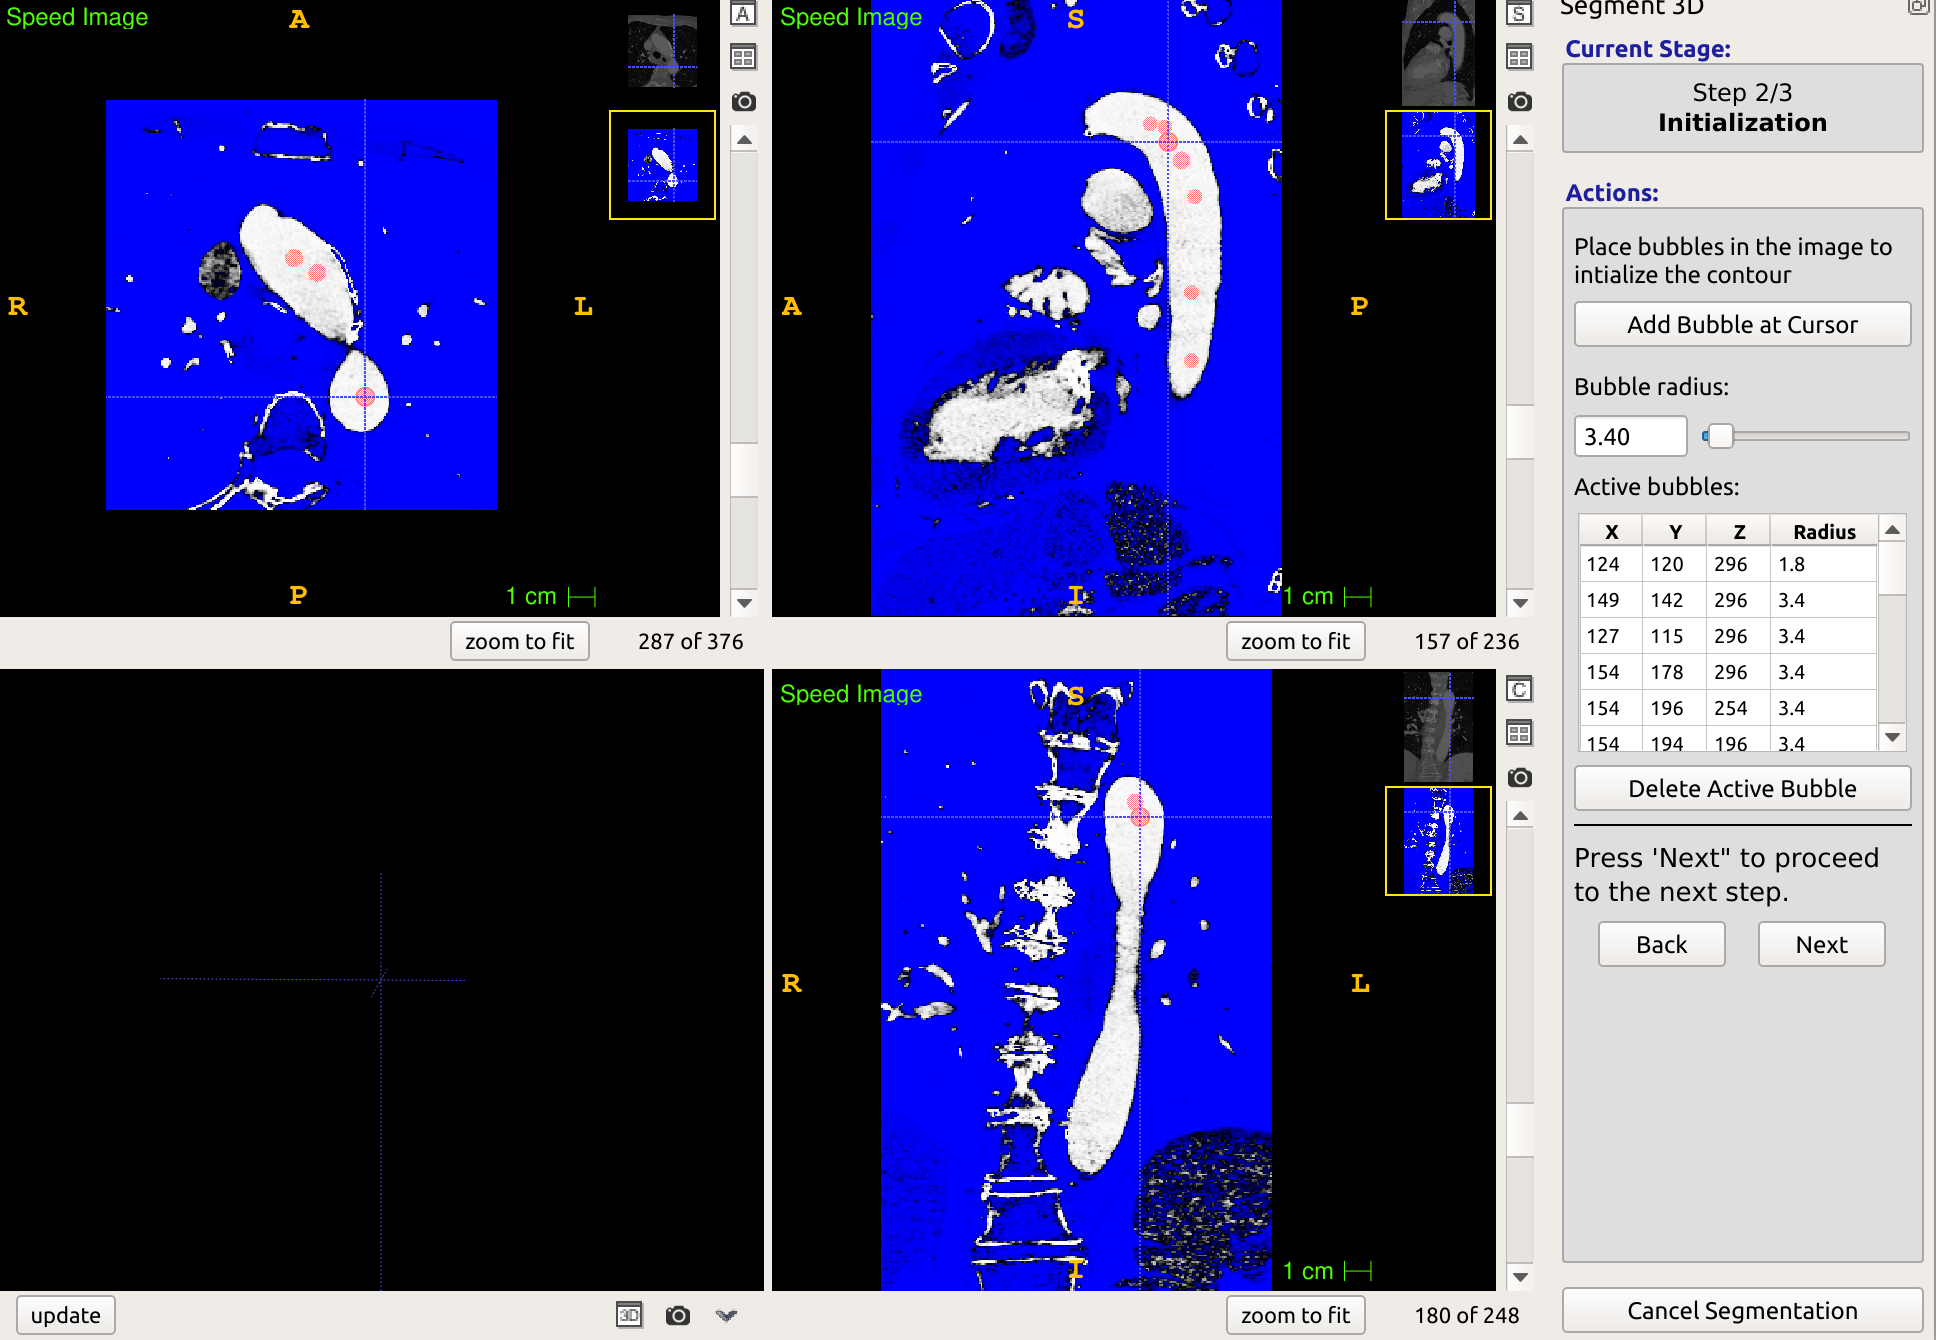
\includegraphics[width=\textwidth]{figures/AGR/bubbles.png}
    \caption[ITK-Snap's Bubble segmentation UI]{ITK-Snap's Bubble segmentation method}
    \label{fig_ITK}
\end{figure}

The advantages of the bubble method is that it guarantee to produce a correct the segmentation result. A medical domain expert can manually control the wanted area, and visually observing the segmentation result expanding, shrinking and the user can erase the unwanted part.

The disadvantages of this method is that the operations described above are complicated. Easier to say then do, an operator who has previous experience building the geometry with this method still needed 20 minutes of manual work building a new aorta geometry. Plus, ITK-Snap software can only read VTK file, therefore the chest CT scans that are usually DICOM, needed a manual conversion before using this software and its segmentation method.

\subsection{3D Slicer threshold segmentation}
3D Slicer is another well-known medical image processing software for academic. 3D Slicer provides multiple segmentation methods, and one of the quickest and easiest to use is the intensity based segmentation.

This method first let user select a small area that belongs to the wanted area on a 2D plane (Axial, Sagittal, and Coronal). 3D Slicer read the pixels' intensity of the surrounding area, and segment based on the intensity threshold. Any pixel's intensity that is within the range will be segmented as the segmentation result. 

Like the bubble method, this method often reads extra volume, and requires user to cut the unwanted parts. A \href{https://www.youtube.com/watch?v=5_673cHMBiY}{YouTube video} shows an experience user who gets the aorta 3D geometry with 8 minutes of manual works. 

\begin{figure}[H]
    \centering
    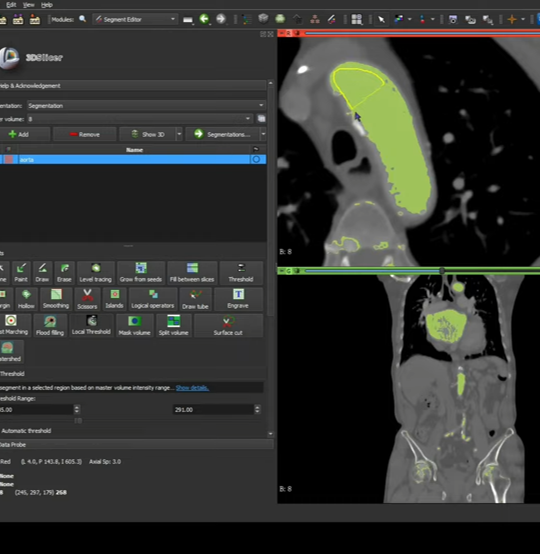
\includegraphics[width=\textwidth]{figures/Sample/3D-Slicer-Segmentation.png}
    \caption[3D Slicer Built-in Segmentation UI]{3D Slicer Built-in Segmentation Method}
    \label{fig_3D_Seg_Builtin}
\end{figure}

\section{Segmentation Algorithm}

This section introduces the key concepts of the implementation on the segmentation algorithm. The algorithm is developed in Python with the external libraries, SimpleITK and NumPy. The algorithm builds the 3D Aorta geometry by doing segmentation on each axial slice. The logic behind segmenting each slice from the axial view, is that there is one or two circles that is edged bounded in each axial plane view. Using this information, and given an initial Aorta center coordination, the algorithm continuously segments each axial's slice circle closest to the previous Aorta center coordinate. Finally, some hyperparameters tuning can let the algorithm pick up the pixels that were missing but belongs to the part of the Aorta.

\subsection{Background} \label{algo_bg}

SimpleITK is an open-source multidimensional image analysis library Developed by the Insight Toolkit community for the biomedical sciences and beyond. NumPy is the fundamental package for scientific computing with Python, especially for the performance on multidimensional array processing. The algorithm will use functions from these two libraries for image processing and multidimensional array processing. For example, the algorithm segments each slice with ThresholdSegmentationLevelSetImageFilter from SITK.

The algorithm works best with the chest volume cropped to a rectangular prism that contains the aorta and parts of the other organs such as the backbone, blood vessels, and the heart. This can be done with 3D Slicer and its built-in modules, Volume rendering and Crop Volume, or researched by the user to find the starting point and the size to crop.

\subsection{Parameters}

At the beginning of the algorithm, the user inputs two integer coordinates indicating the position of the descending aorta and ascending aorta center on a single slice. The yellow dots in Figure ~\ref{fig_aorta_seed} shows an example of the aorta seeds. These seeds will be updated by the algorithm after processing each axial plane.

\begin{figure}[ht]
    \centering
    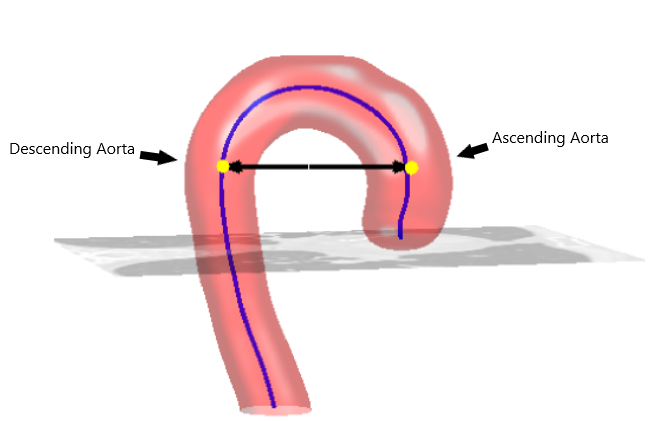
\includegraphics[width=0.7\textwidth]{figures/Sample/Aorta_seeds.png}
    \caption[The Aorta Seeds]{The aorta seeds \citep{6346433}}
    \label{fig_aorta_seed}
\end{figure}

On the other hand, this list of hyperparameters that can be tuned to get the best segmentation result:
\begin{itemize}
\item The stop limit which controls the stop condition
\item The threshold coefficient which controls the segmentation acceptable intensity range
\item The kernel size which controls the label image circle size 
\item The threshold Segmentation Level Sets Image Filter parameters, including:
\begin{itemize}
\item The RMS error
\item The maximum iteration
\item The curvature scaling
\item The propagation scaling
\end{itemize}
\end{itemize}

One of the most important parameters is the threshold coefficient. Since the algorithm segments based on the intensity of the gray scale pixels, decreasing the threshold coefficient would decrease the acceptable range of the pixels, and vice-versa. 


\subsection{Algorithm Overview} \label{algo}

When the user has selected the aorta seeds, the plane where the aorta seeds located is the initial plane. From this plane towards the bottom (the feet) is inferior direction. On the other hand, it is superior direction. This algorithm segments each slice with SITK::ThresholdSegmentationLevelSetImageFilter. The principles of this image filter can be explained with two terms: Level sets segmentation method, and a threshold range that defines the intensity of the acceptable pixel.

Level Sets are an important category of modern image segmentation techniques based on partial differential equations (PDE), i.e. progressive evaluation of the differences among neighboring pixels to find object boundaries. The pictures~\ref{LSS} demonstrate an example of how Level Sets method work on finding the region of the heart. It starts with a seed contour that is within the region of interest, then by finding the gradient based on the contour line, the segmentation result will propagate towards outside the region until the maximum difference between the neighboring pixels are reached.

\begin{figure}[H] 
\centering
\subfloat[\centering Init image]{{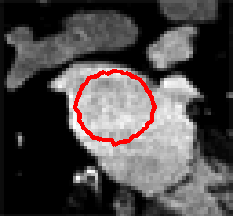
\includegraphics[width=0.33\textwidth]{figures/AGR/heart-1.png}}}%
\subfloat[\centering Expanding]{{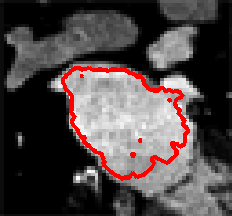
\includegraphics[width=0.33\textwidth]{figures/AGR/heart-2.png}}}%
\subfloat[\centering Result]{{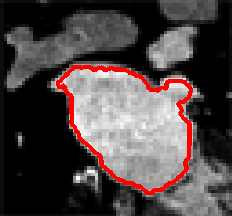
\includegraphics[width=0.33\textwidth]{figures/AGR/heart-3.png}}}%
\caption{Level Sets Segmentation}
\label{LSS}
\end{figure}

\subsection{The steps to segment a single slice}
In the following section, we will present each step to segment a single slice. These steps applied in both segmentation in superior and inferior direction, there is a difference in the stop condition, which we will elaborate in the following section.
\subsubsection{Create A Label Map}
The algorithm uses SITK::BinaryDilateImageFilter to perform binary dilation to generate a circle-like shape around the center coordinates (user input’s for the first slice and calculated by the algorithm for the rest of the slices). Each pixel within this shape will be labeled as a white pixel (value of 1), and the rest of the pixels are labeled as black pixels (value of 0). 

The generated result is the label map image, and we will use it in the next few steps. The size of the circle-like shape is determined by the kernel size (user's input). The Figure \ref{fig_label_map} shows an example of generated label map image (the green parts) overlay over the original slice.

\begin{figure}[H]
    \centering
    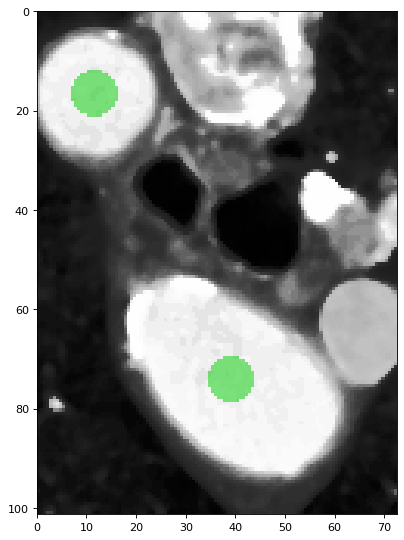
\includegraphics[width=0.5\textwidth]{figures/AGR/label_image.png}
    \caption[A label image]{A label map}
    \label{fig_label_map}
\end{figure}

\subsubsection{Create A Distance Map}\label{distance_map}
With SITK::SignedMaurerDistanceMapImageFilter, the algorithm creates another image, the Euclidean distance transform of the label image from previous step. This is used as a contour line that helps build the gradient mentioned in Level sets. The Figure \ref{fig_distance_map} shows an example of distance map.

\begin{figure}[H]
    \centering
    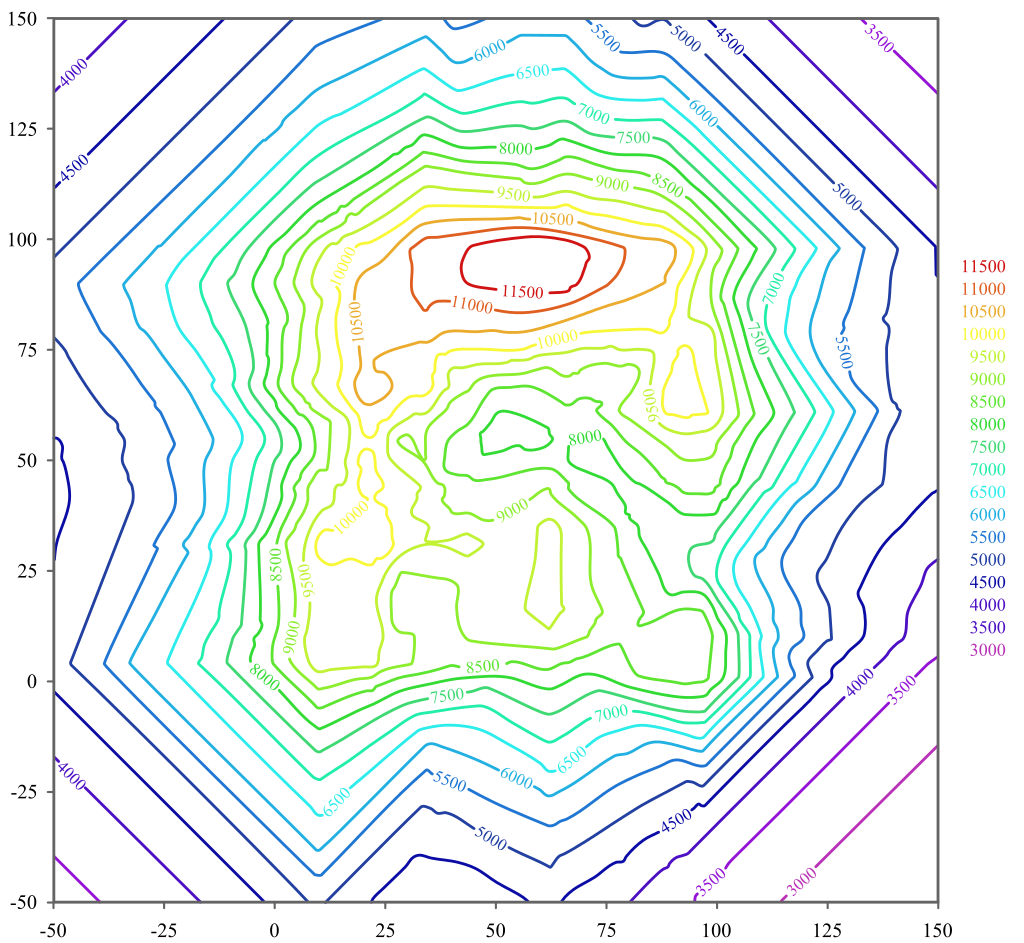
\includegraphics[width=0.5\textwidth]{figures/AGR/Contour2D.png}
    \caption[A distance map]{A distance map}
    \label{fig_distance_map}
\end{figure}

\subsubsection{Calculate a threshold range} \label{threshold}
By using SITK::LabelStatisticsImageFilter, the algorithm gets the mean and the standard deviation of the intensity values of the pixels that were labeled as the white pixel in the label map. The algorithm uses threshold coefficient to calculate the lower and upper threshold to be used in the next step.

\begin{figure}[H]
    \centering
    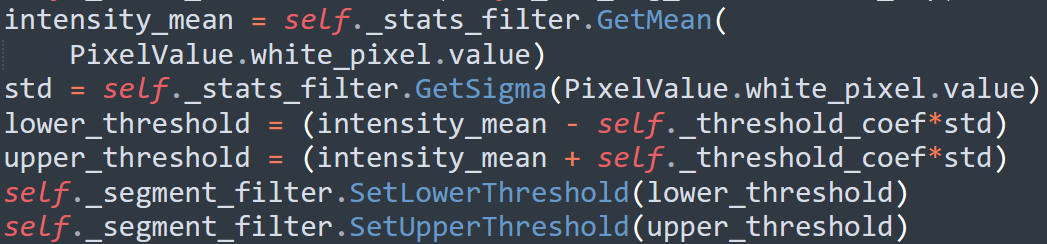
\includegraphics[width=\textwidth]{figures/AGR/threshold.png}
    \caption[Code that shows how to calculate the threshold range]{Code snippet shows the intensity threshold calculation}
    \label{fig_threshold}
\end{figure}

\subsubsection{Segment a single slice}
With SITK::ThresholdSegmentationLevelSetImageFilter, the seed image calculated in step \ref{distance_map}, and the lower and upper threshold value calculated in step \ref{threshold}, the algorithm performs segmentation and generated a segmented slice. The Figure~\ref{fig_segmented_image} shows an example of generated segmented slice (the green parts) overlay over the original slice.

\begin{figure}[H]
    \centering
    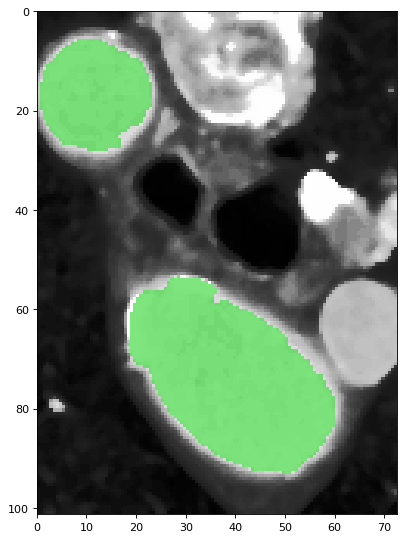
\includegraphics[width=0.5\textwidth]{figures/AGR/segment_label_image.png}
    \caption[A segmented image]{A segmented image on top of the original slice}
    \label{fig_segmented_image}
\end{figure}

\subsubsection{Calculate new centroids}
By comparing each pixel segmented as aorta to the previous descending centroid and the previous ascending centroid, the algorithm use the positions of the points closer to the previous descending centroid to calculate new descending aorta centroid, and vice-versa for the ascending aorta centroid. However, at certain point during the segmentation in inferior direction, the slice might reach the end of the ascending aorta, the Aortic Root, the algorithm will stop using and calculate ascending aorta centroid and only computes descending aorta centroid for the slices afterward.

\subsubsection{Verify segmentation result}
There are two main stop conditions for verifying segmentation result, one condition for the segmentation in inferior direction and the other one for the segmentation in superior direction. Stop limit is a user defined parameter to control the algorithm, to calculate the condition with the centroids position and the standard deviation.

In inferior direction, if the new ascending aorta centroid that is closest to the previous ascending aorta center is reaching the distance limit, then the algorithm will stop consider taking the new centroid closer to the ascending aorta. In other words, only 1 centroid will be used for descending aorta segmentation.

In superior direction, if the standard deviation of the initial label map and the segmentation result label map has larger difference than the limit, the algorithm will stop processing segmentation for the rest of the slices. For example, assume that the standard deviation of the initial label image is 20, and the standard deviation of the segmentation label image is 40, with stop limit of 10, the program halt immediately.

\subsection{Algorithm Summary}
Given two integer coordinates, ascending aorta centroid and descending aorta centroid, the algorithm set the inputted plane as the initial plane. From the initial plane to the bottom (the feet) plane, the algorithm calculate a label map with two centroid coordinates and kernel size, calculate a distance map with the label map, calculate a threshold range with the label map's selected pixels, perform segmentation, calculate new centroid coordinates, and verify the segmentation result in case that it reaches the stop condition. Once the algorithm finished the segmentation in inferior direction, the algorithm works from the initial plane to the top (the head) plane, repeating the similar steps. Each segmentation result slice is stored in a SITK's image, which supports the conversion to VTK file or DICOM file.

\begin{figure}[H]
    \centering
    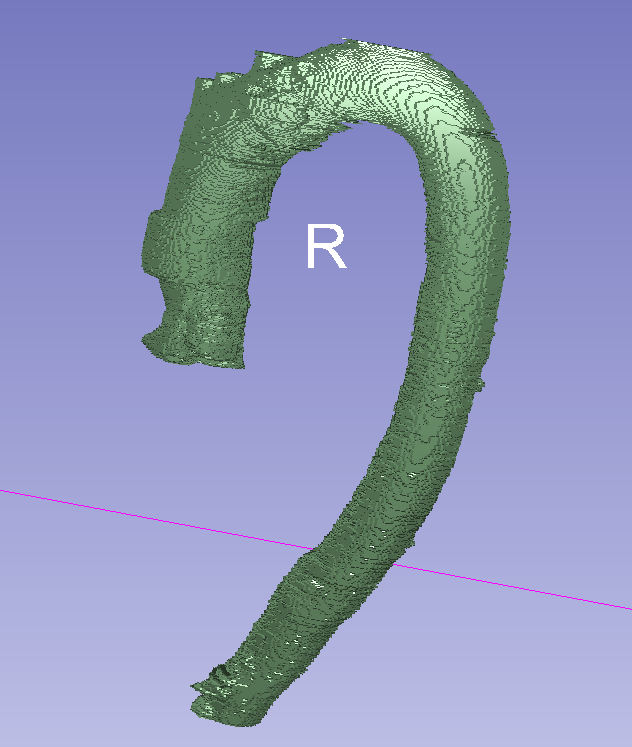
\includegraphics[width=0.5\textwidth]{figures/AGR/segmentation_result.png}
    \caption[Segmentation Result]{Segmentation Result}
    \label{fig_sr}
\end{figure}

\section{3D Slicer Extension Development}
The project has started with a simple segmentation algorithm build on the Jupyter notebook. When getting a new patient's data, the user will need to investigate the chest ct scans using another software (3D Slicer, ITK-Snap), to get the readings such as coordinates and size to crop (the coordinates of the yellow dots shown in Figure~\ref{fig_aorta_seed}).

\begin{figure}[H]
    \centering
    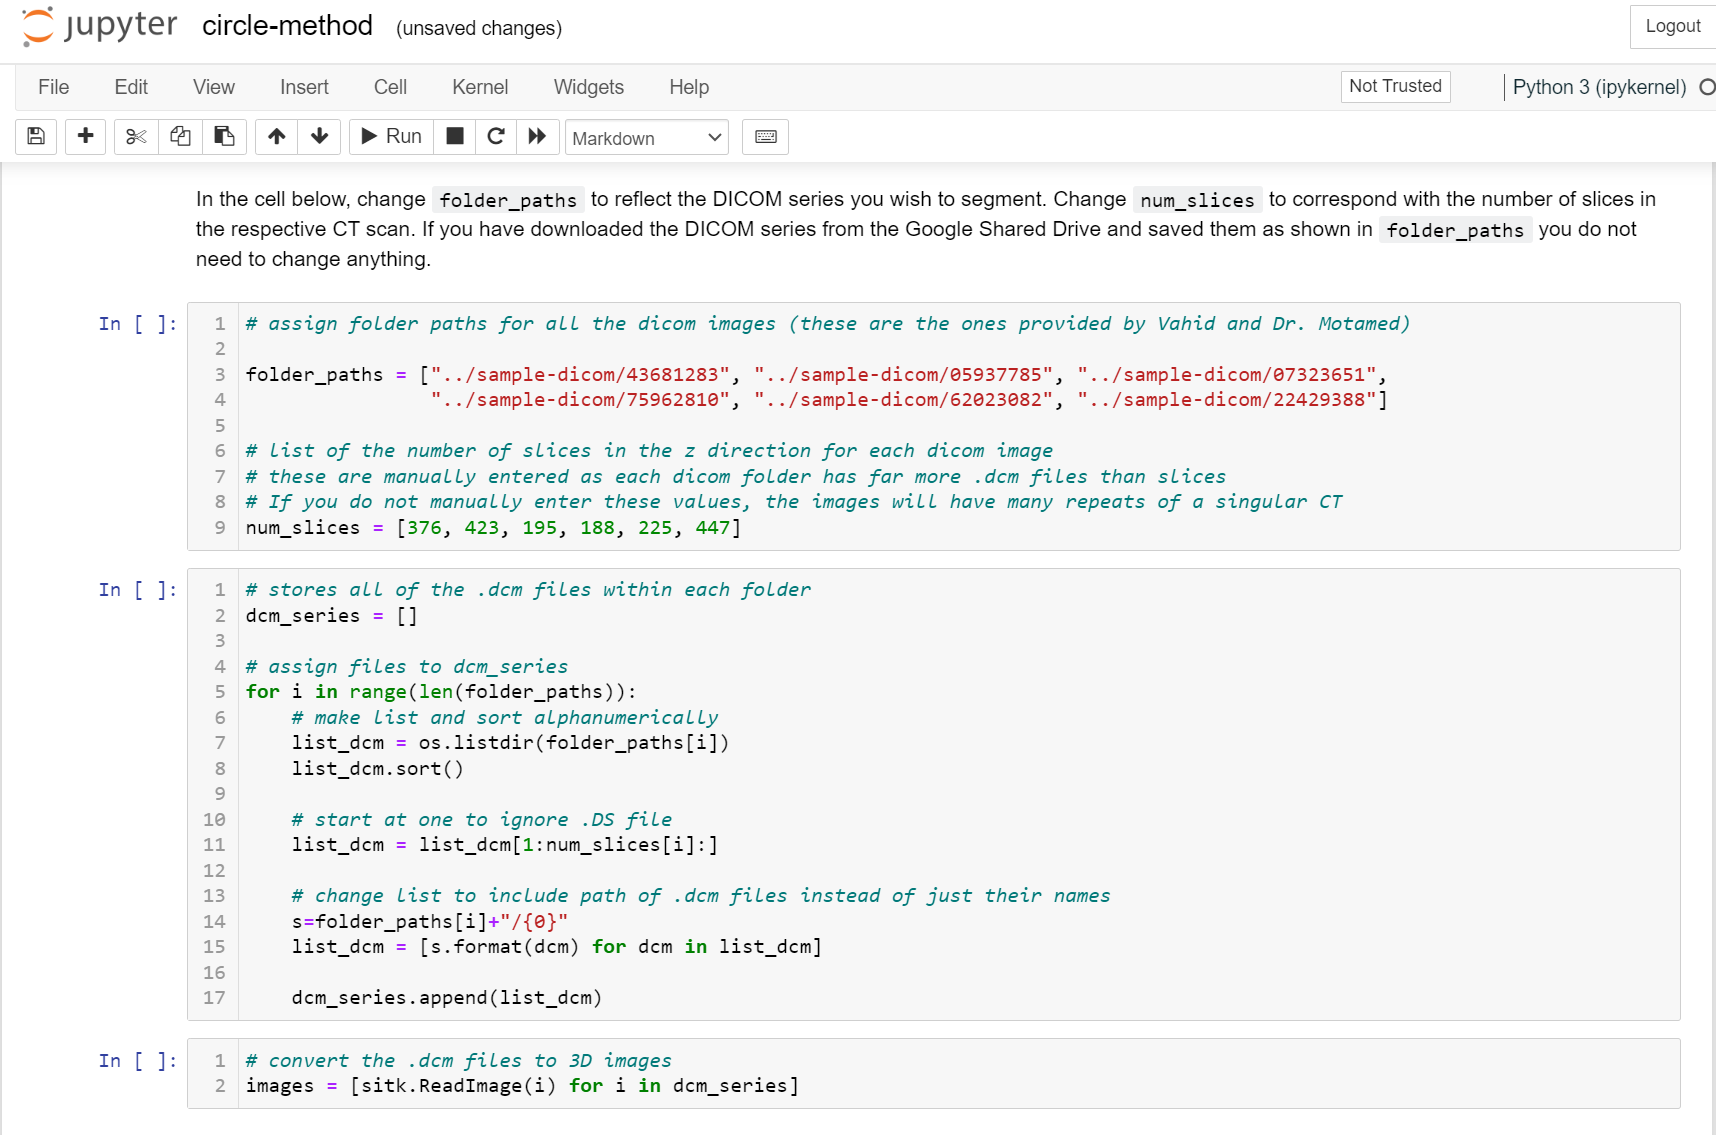
\includegraphics[width=\textwidth]{figures/AGR/jupyter_research.png}
    \caption[Jupyter Notebook Research]{Jupyter Notebook Researched by Kailin Chu}
    \label{fig_jnr}
\end{figure}

Originally, the parameters entered by the users, and many other values are hard-coded in the Jupyter Notebook. To improve the usability of the \progname{} (reduce the amount of time for user inputs and execution), we implemented an extension module on 3D Slicer. 

3D Slicer is an open-sourced medical image processing software for research. 3D Slicer provides useful modules such as Crop Volume module and Volume Rendering module that easily crop any volume. 3D Slicer is highly modulable with Python scripting to control the extension module sequence, and QT designer to generate Graphical User Interface.

%\begin{figure}[ht]
%    \centering
%    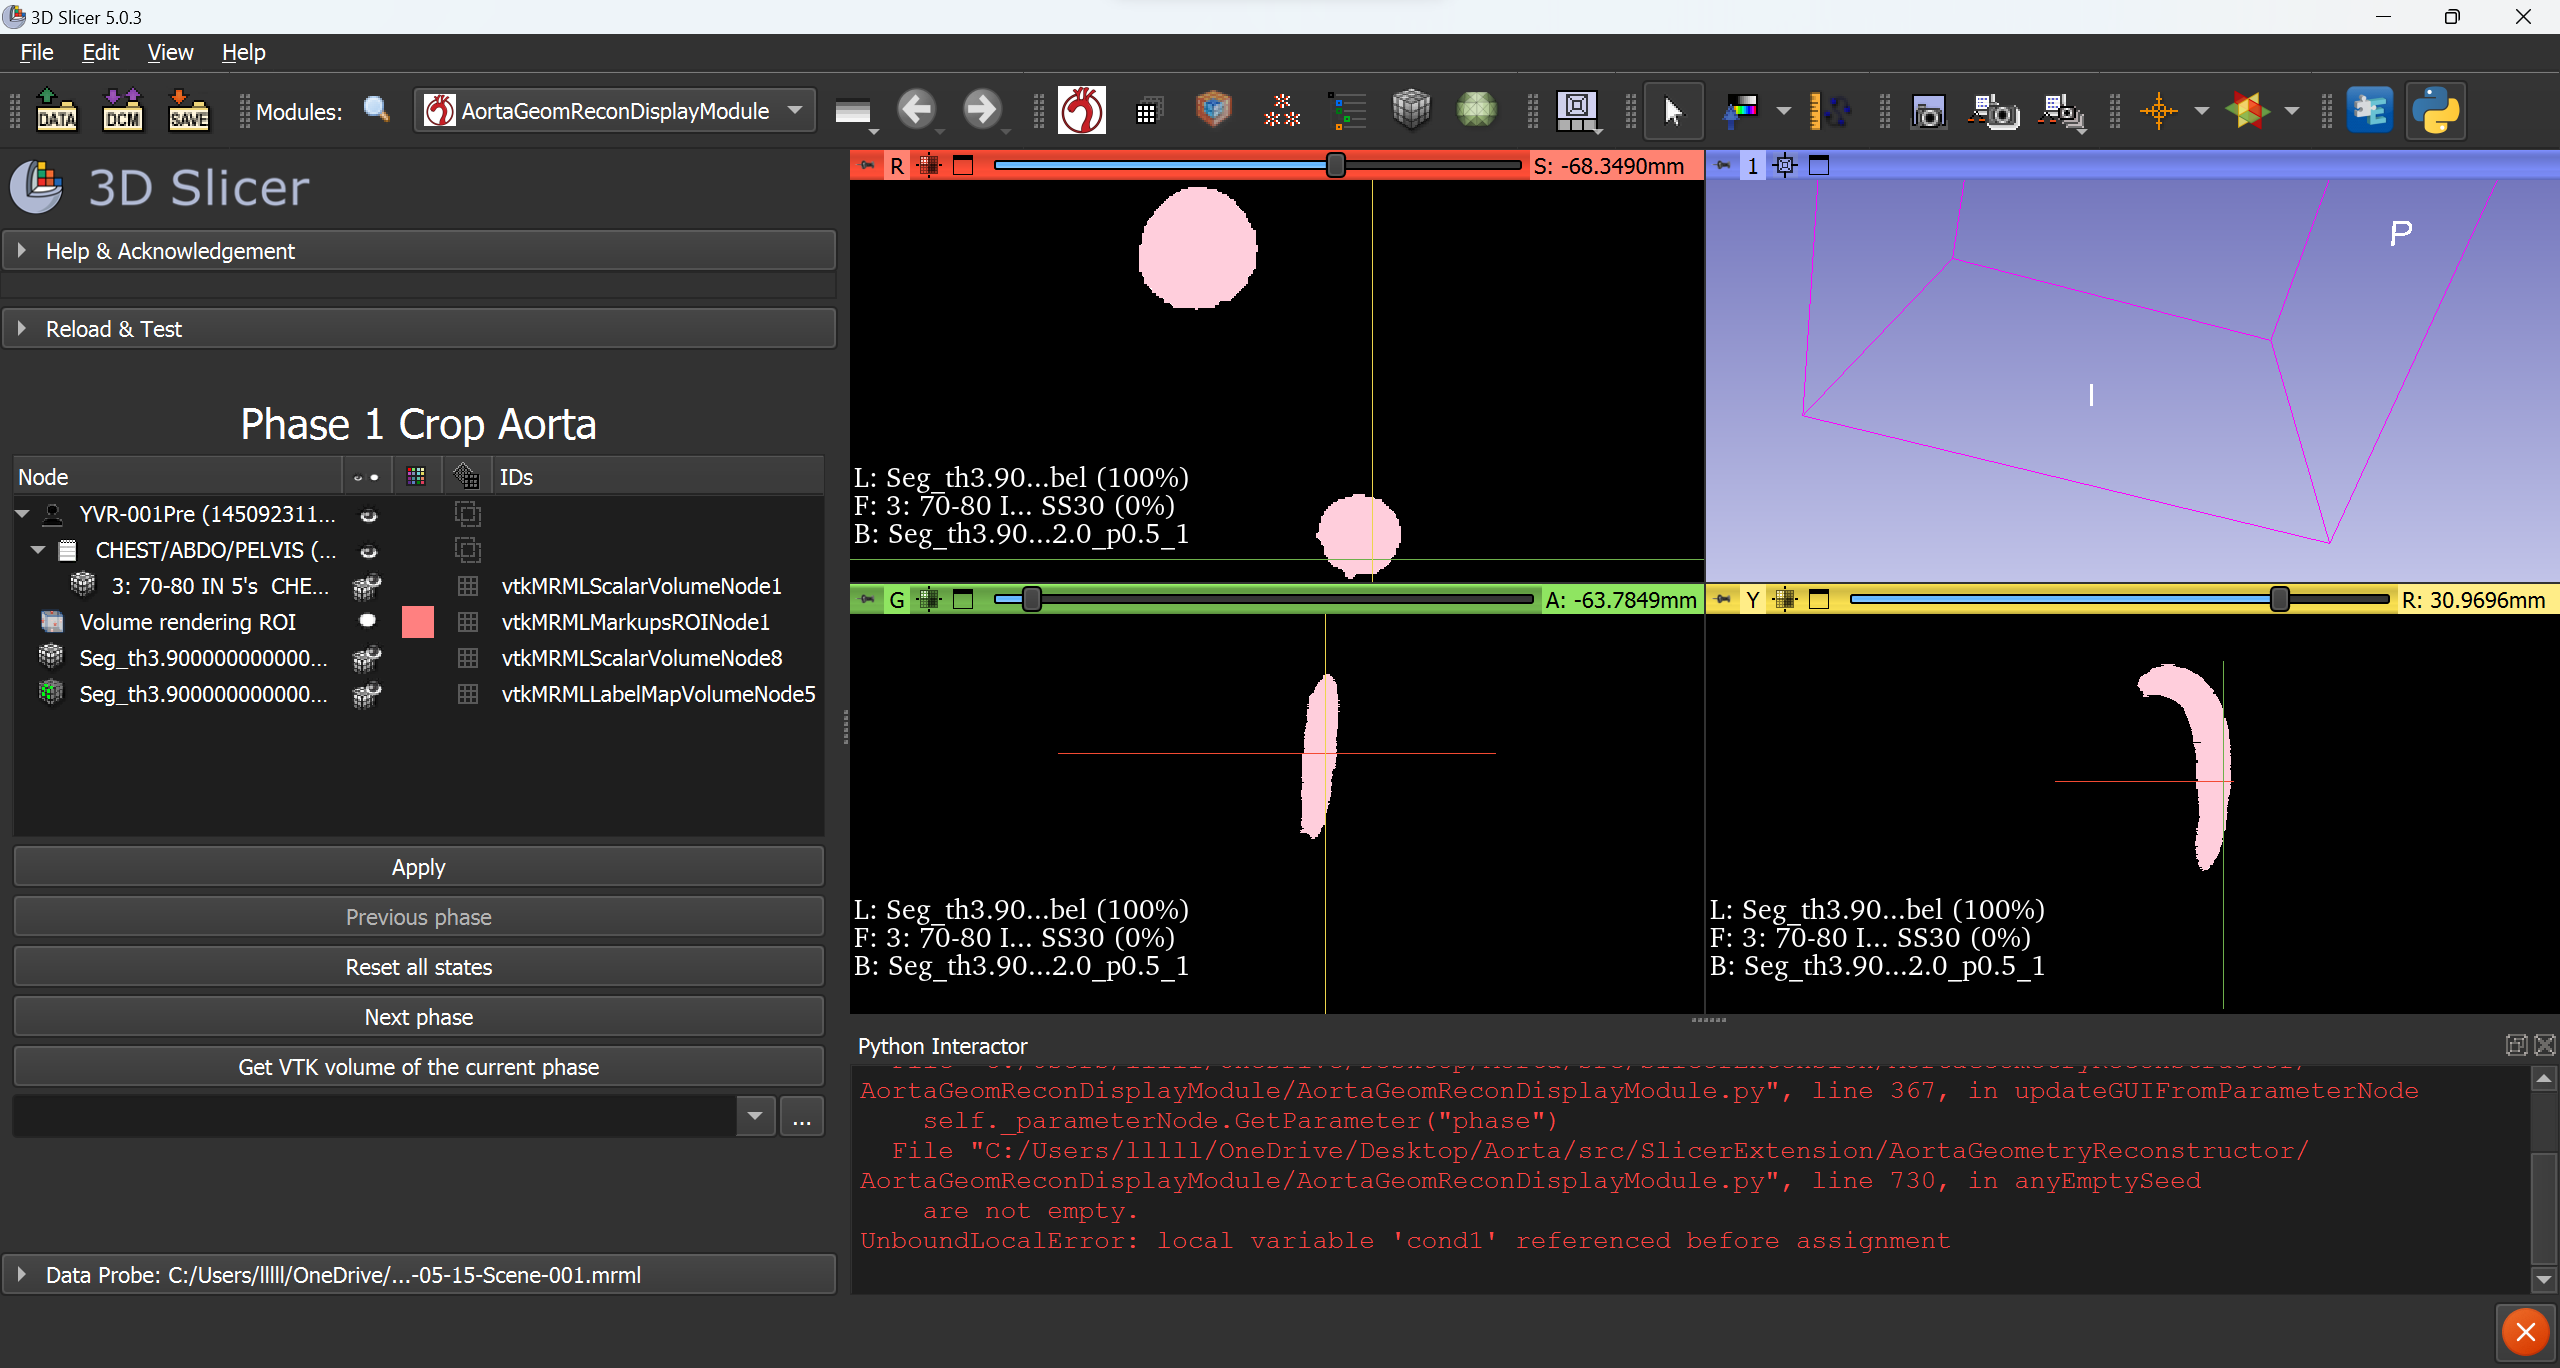
\includegraphics[width=\textwidth]{figures/Sample/SlicerUI.png}
%    \caption[AortaGeomRecon phase 1 User Interface]{AortaGeomRecon UI phase 1}
%    \label{fig_UI_1}
%\end{figure}
%
%\begin{figure}[ht]
%    \centering
%    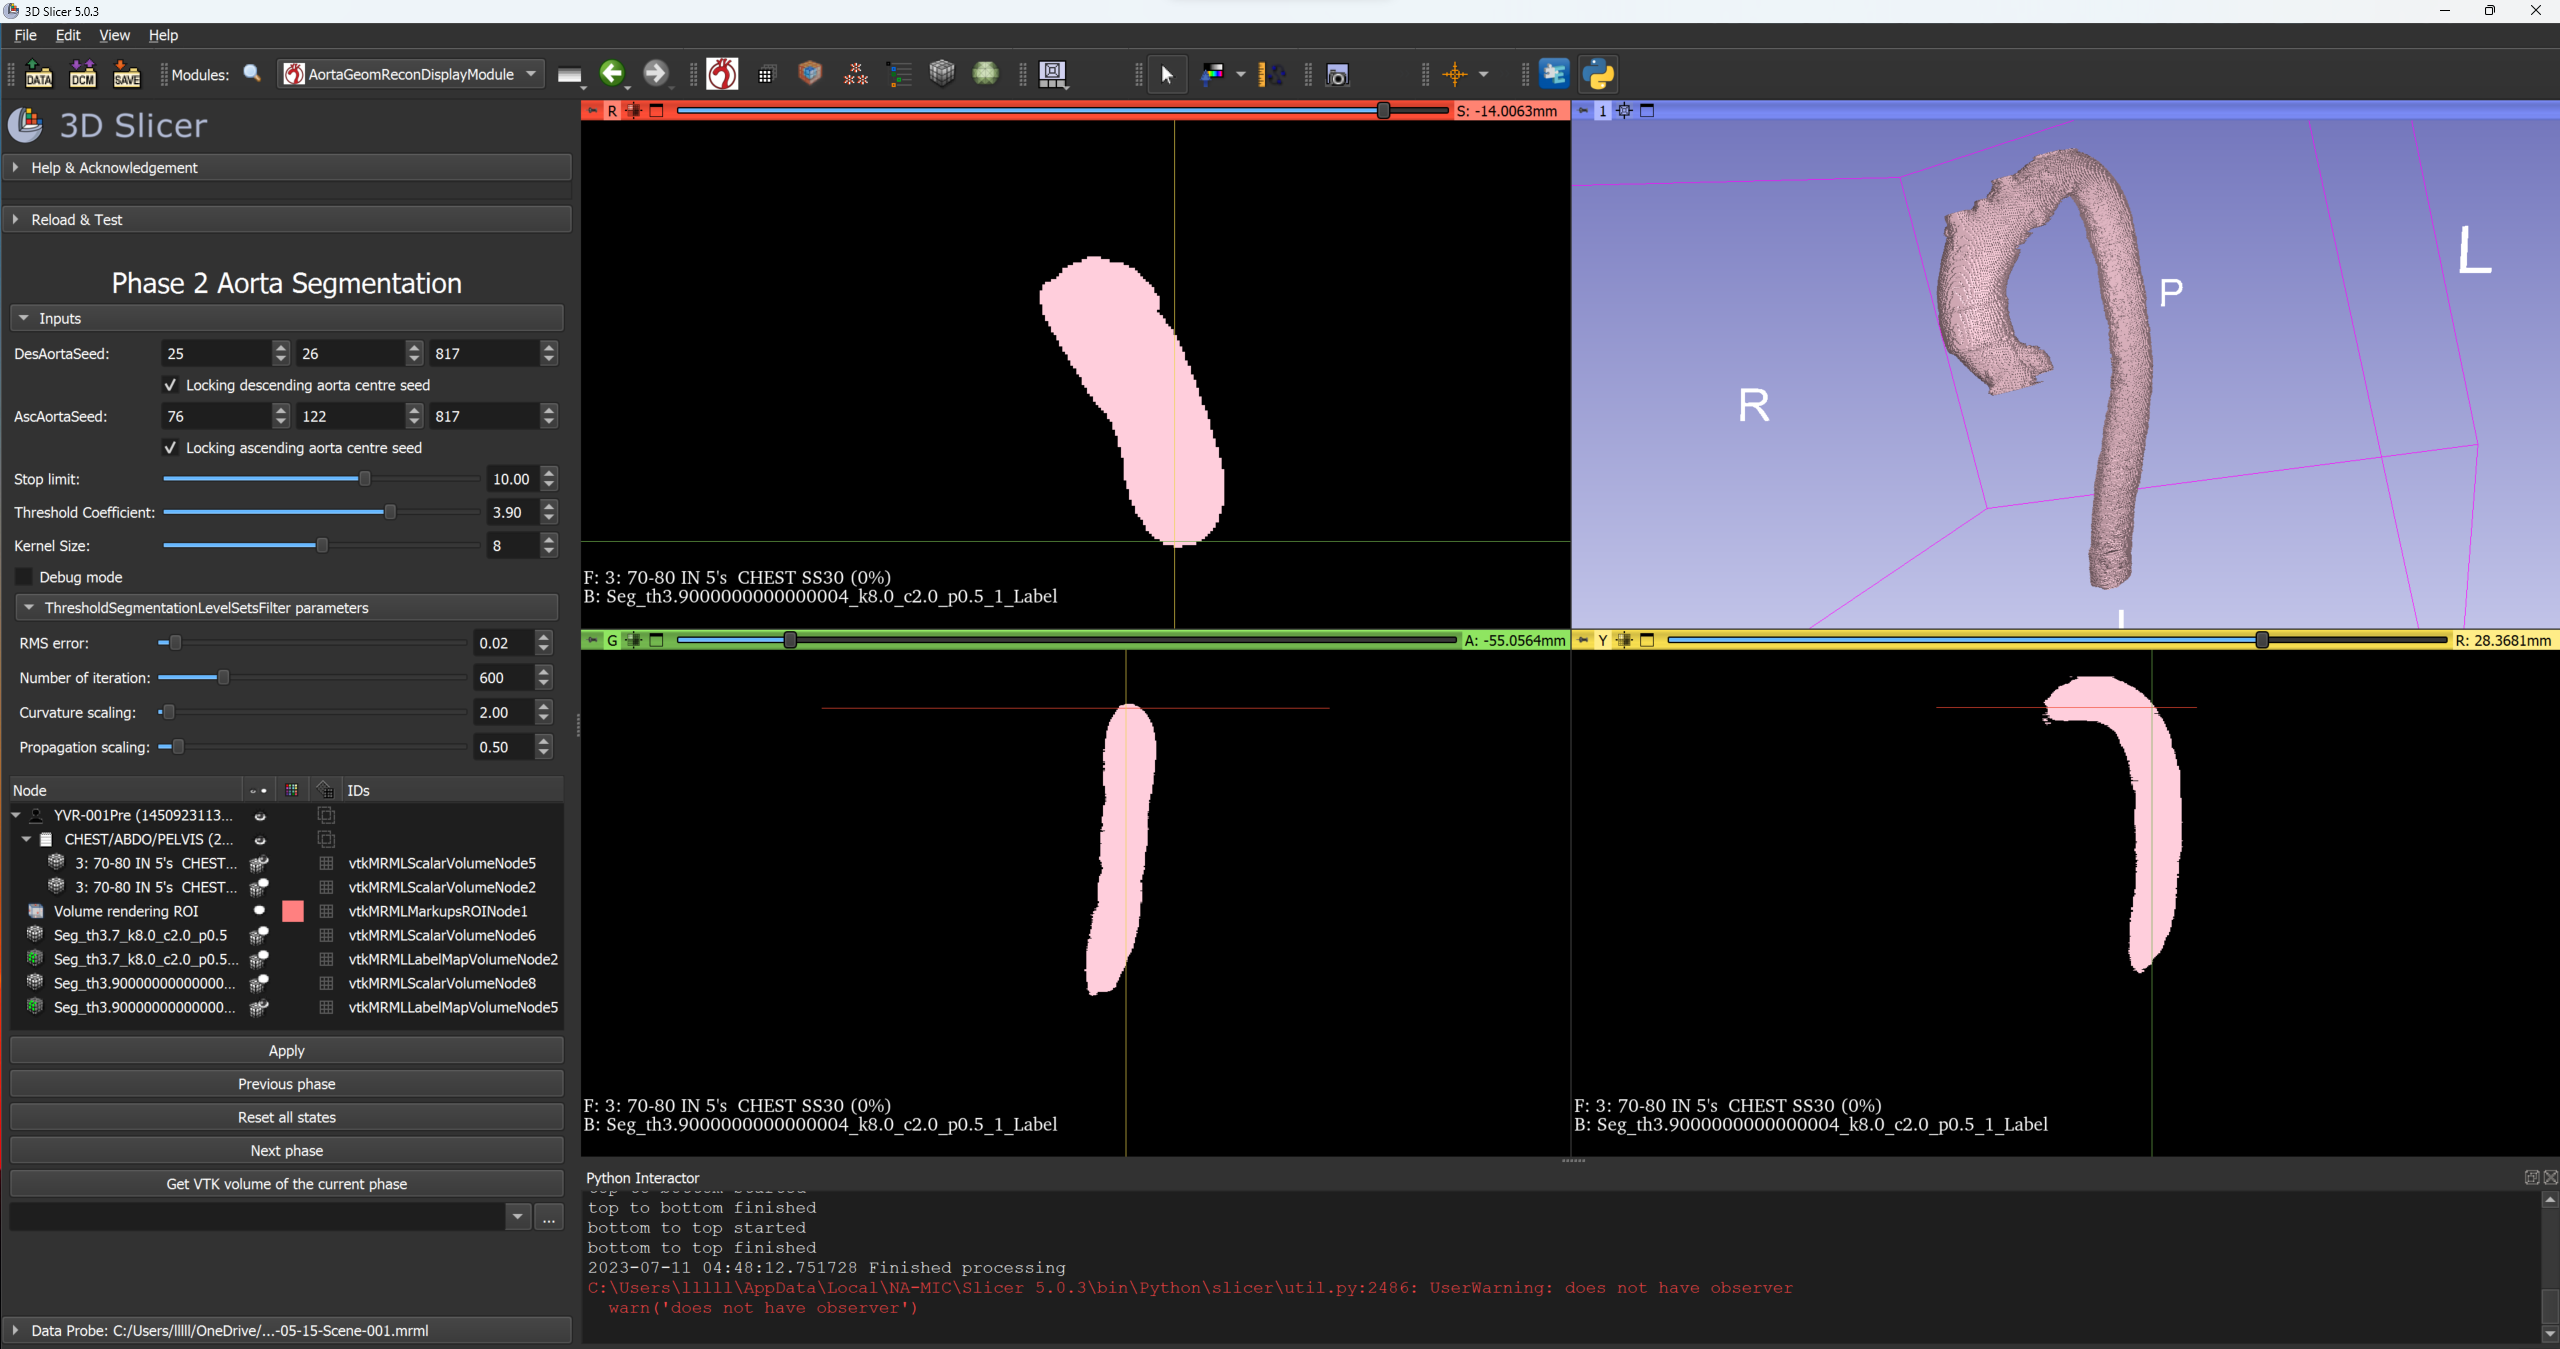
\includegraphics[width=\textwidth]{figures/Sample/SlicerUI_2.png}
%    \caption[AortaGeomRecon phase 2 User Interface]{AortaGeomRecon UI phase 2}
%    \label{fig_UI_2}
%\end{figure}

3D Slicer supports modularization with an extension. An extension can compose multiple modules, where each module is dedicated to solve a sub-problem.
%\begin{itemize}
%\item 3D Slicer Data Structure \\ 
\subsection{3D Slicer's data structure}

3D Slicer's Data Structure can be divided into two categories. The Node data structure store large data such as DICOM with a Volume Node, Volume rendering Region of Interest Node, Label Map Volume Node. The parameters are stored as string from the UI component of the module. Every data stored in 3D Slicer can be accessed by the 3D Slicer's Widget Class and Logic Class for further processing. 

3D Slicer stores all the above data in a scene object, which is also referred as MRMLscene file, on the higher level data format. 3D Slicer can load any MRMLscene file, this allowed user to retrieve all the data nodes and parameters. On the other hand, 3D Slicer has a special input module, the DICOM database allowed user to store DICOM metadata in 3D Slicer.

\subsection{3D Slicer's scripted module}

Every ScriptLoadableModule in 3D Slicer have a Widget Class and a Logic Class. The Widget Class is used to initialize the extension module's UI component, and the parameters tied to the UI component. The module's Logic Class is used to perform the processing of the data. In the Logic Class, we initialize an AortaGeomRecon Segmenter object with the attributes set to the parameters reading from UI component, which are inputs by the user. After completing the segmentation with Segmenter object, we convert the SimpleITK image object to a volume node corresponding in 3D Slicer, which allow the user to visualize the segmentation result. 

\subsection{AortaGeomReconDisplayModule}
\subsubsection{Graphical User Interface}

\begin{figure}[H]
    \centering
    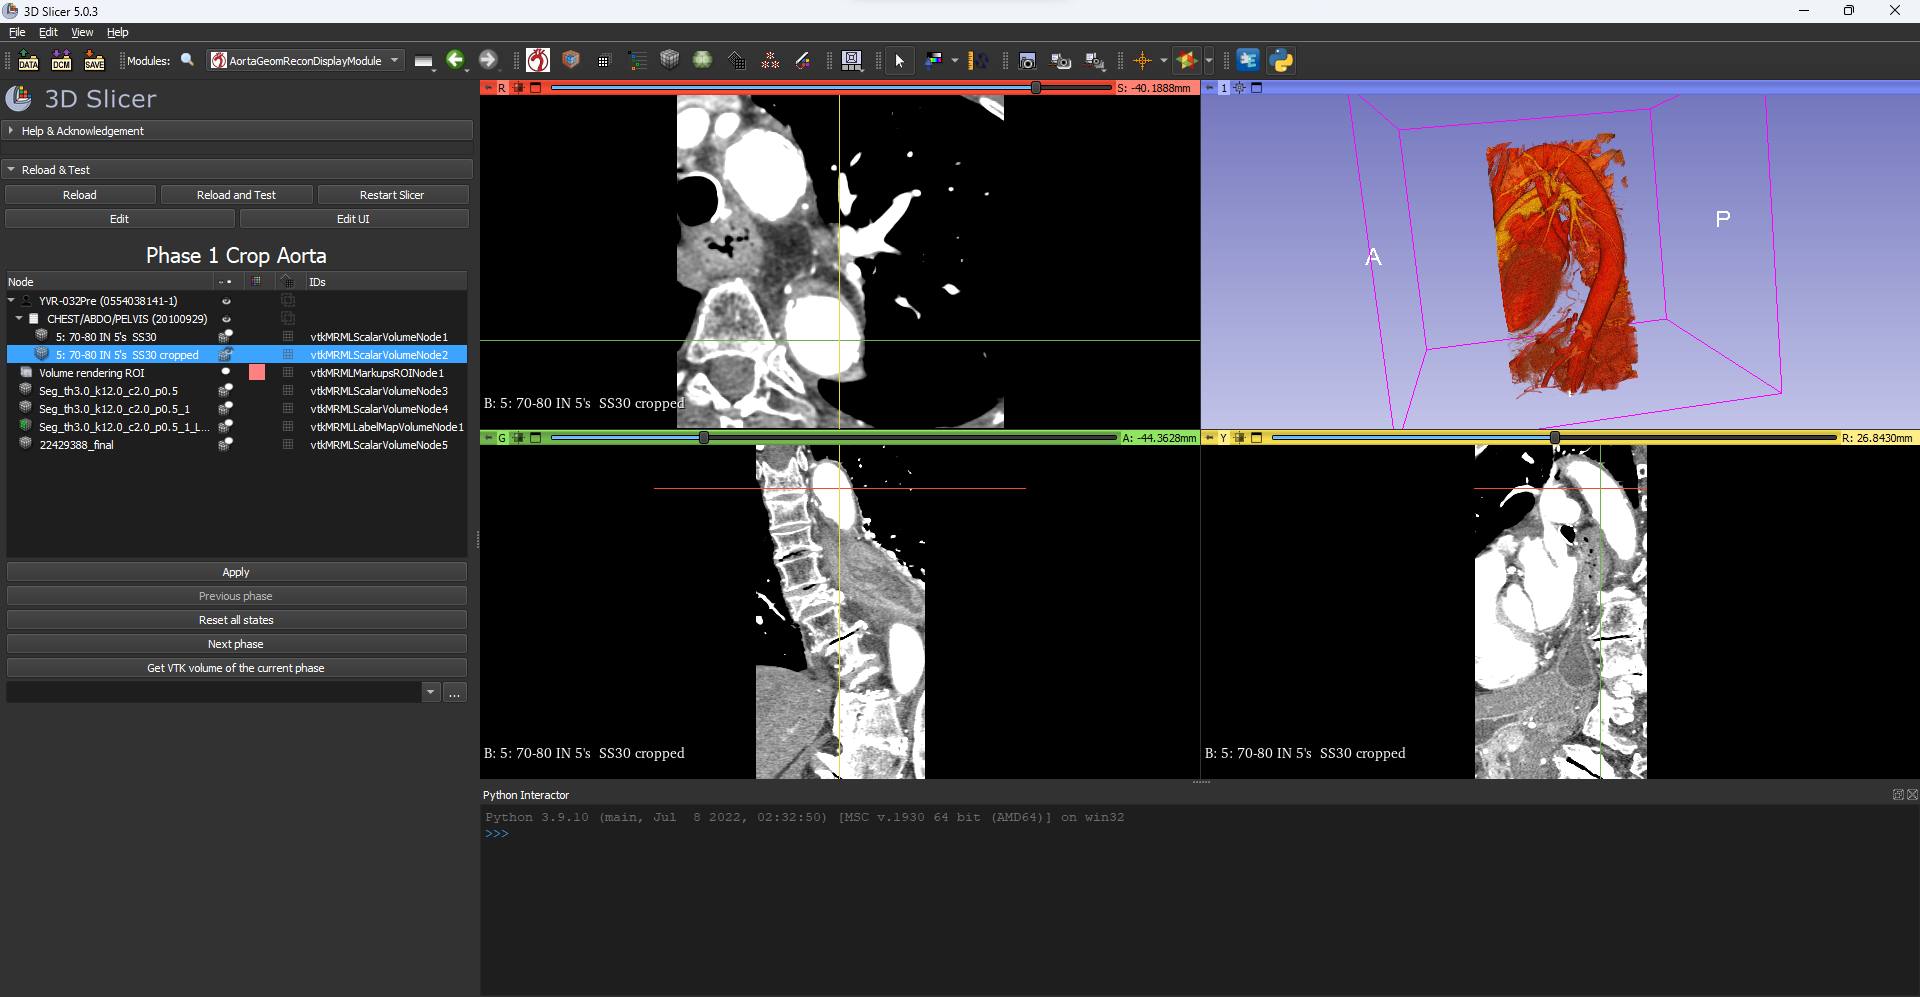
\includegraphics[width=\textwidth]{figures/AGR/Slicer_UI.png}
    \caption[3D Slicer UI]{3D Slicer UI}
    \label{fig_slicer_ui}
\end{figure}

3D Slicer separate the UI into two parts. From the Figure~\ref{fig_slicer_ui}, we can see that the four windows on the right side of the UI are used to visualize a volume. The left side shows the SubjectHierarchyTreeView which the module already stored many data nodes. The first node is the DICOM patient data with the chest CT scans stored as a volume, and the cropped volume I generated with Crop Volume Module. There is a Volume rendering ROI node and several ScalarVolumeNode which are the generated segmentation volume with different parameters.

The left side is the module UI. This part is designed and implemented differently based on the requirements of the modules. The Figure~\ref{fig_module_ui} shows the module UI that the AGR implemented, where each parameter stored to be passing to the algorithm class.

\begin{figure}[H]
    \centering
    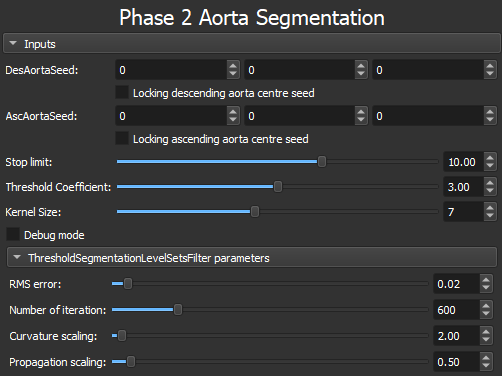
\includegraphics[width=\textwidth]{figures/AGR/Module_UI.png}
    \caption[AortaGeomRecon Module UI]{AortaGeomRecon Module UI}
    \label{fig_module_ui}
\end{figure}


\subsubsection{Module's Workflow} \label{module_workflow}
When the user first starting 3D Slicer and click on the AGR module, this warning message and Tips appears in the module UI. The user must click on the confirm button below to proceed into the next steps. This warning message is an evidence for the assurance case, which I will explain in the next chapter.

\begin{figure}[H]
    \centering
    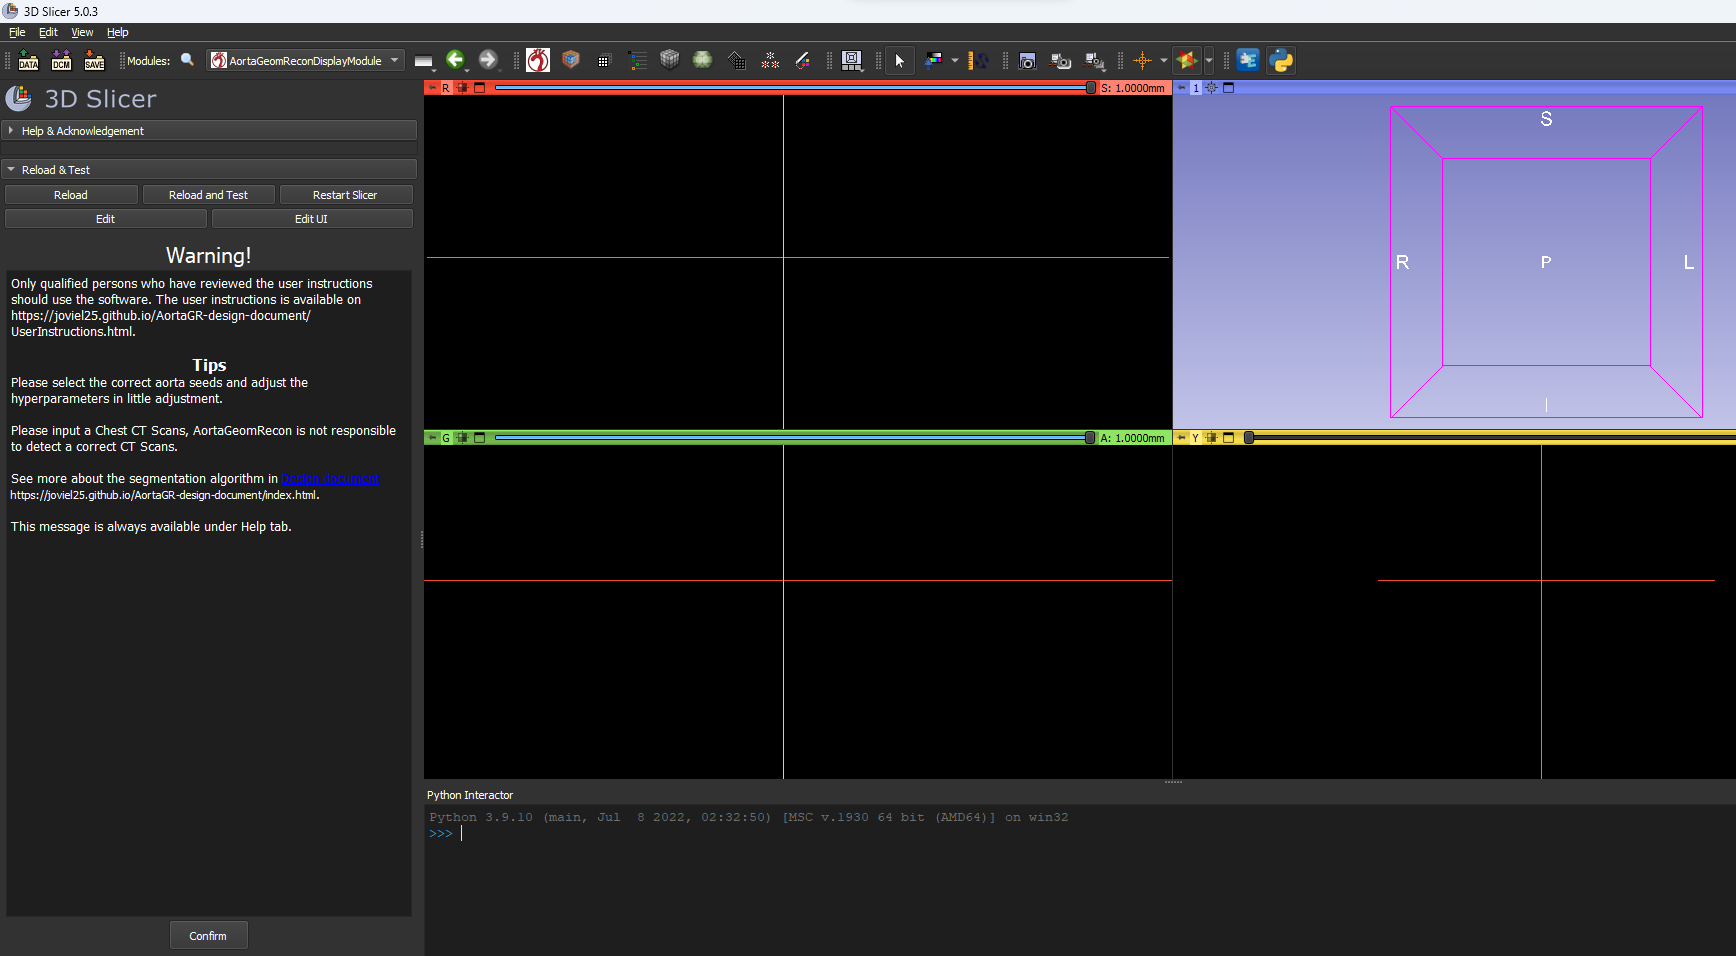
\includegraphics[width=\textwidth]{figures/AGR/AGR_warning.png}
    \caption[AortaGeomRecon Warning message]{AortaGeomRecon Warning message}
    \label{fig_agr_warning}
\end{figure}

In the next step, assuming that the user has already read a DICOM image of the patient's chest, the user is asked to generate a cropped volume using the 3D Slicer's Volume Rendering module and the Crop Volume module. In this phase, the module UI displays only a SubjectHierarchyTreeView where the large data node are shown in this view. After generated a cropped volume, the apply button is enabled and the user can proceed to the next step.

In phase 2 aorta segmentation, the user is asked to input the parameters to perform the segmentation. The module UI is same as the Figure~\ref{fig_module_ui}. The necessary inputs are the two aorta seeds, without any value for these two inputs, the module will not allow user to generate segmentation result.

%\section{GitHub and Workflows}
%This project uses GitHub for version control. \\
%We used GitHub 
%
%GitHub issues tracker use to keep track the items to work on throughout the development of the project\\
%GitHub Project is used for dividing a large issue into smaller tasks, expected date of the completion. This is useful for project management.\\
%GitHub Workflow is a great tool for Continuous Integration tests. \\
%We uses GitHub Workflow for Linter and Continuous Integration tests. 

%\end{itemize}


%\begin{itemize}
%\item Inputs Parameter


%\item Threshold
%\item LevelSets
%\item Stop Condition
%\end{itemize}
%This is a sample chapter
%
%If you need to use quotes, type it ``like this''.


%\section{Referencing}
%These are some sample references to GAMYGDALA~\citep{popescu2014gamygdala} from 
%the \texttt{references.bib} file and state effects of 
%cognition~\citep{hudlicka2002time} from the \texttt{references\_another.bib} 
%file. These references are not in the same .bib file.
%
%\section{Figures}
%This is a single image figure (Figure~\ref{fig_singleenv}):
%
%\begin{figure}[ht]
%    \centering
%    
\includegraphics[width=0.6\textwidth]{figures/Sample/tumblr_static_eaceks0rfxsss8o4swscw40wo.jpg}
%    \caption[Single Figure Environment Listed Title]{This is a single figure 
%    environment}
%    \label{fig_singleenv}
%\end{figure}
%
%This is a multi-image figure with a top (Figure~\ref{fig_multienv_1}) and bottom (Figure~\ref{fig_multienv_2}) aligned subfigures:
%
%\begin{figure}[ht]
%	\centering
%	\begin{subfigure}[t]{\textwidth}
%		\centering
%		
%
\includegraphics[width=0.7\textwidth]{figures/Sample/tumblr_static_eaceks0rfxsss8o4swscw40wo.jpg}
%		\caption{Figure 1}
%		\label{fig_multienv_1}
%	\end{subfigure}
%	~
%	\begin{subfigure}[t]{\textwidth}
%		\centering
%		
%
\includegraphics[width=0.7\textwidth]{figures/Sample/tumblr_static_eaceks0rfxsss8o4swscw40wo.jpg}
%		\caption{Figure 2}
%		\label{fig_multienv_2}
%	\end{subfigure}
%	
%	\caption{A Multi-Figure Environment}
%	\label{fig_multienv}
%\end{figure}
%
%\section{Tables}
%
%Here is a sample table (Table~\ref{tab_sample}):
%
%	\begin{table}[ht]
%	\centering
%	\begin{tabular}{ m{0.2\textwidth} m {0.1\textwidth} m{0.15\textwidth} }
%		\toprule
%		A & $\longleftrightarrow$ & B \\
%		C & $\longleftrightarrow$ & D \\
%		\bottomrule	
%	\end{tabular}	
%	\caption{A sample table}	
%	\label{tab_sample}
%\end{table}
%
%\subsection{Long Tables}
%A sample long table is shown in Appendix~\ref{appendix_b}.
%
%\section{Equations}
%
%Here is a sample equation (Equation~\ref{eq_lineslope}):
%
%\begin{equation} \label{eq_lineslope}
%	y = mx + b
%\end{equation}